% UTF-8 encoding
% Compile with latex+dvipdfmx, pdflatex, xelatex or lualatex

\documentclass[hyperref, UTF8]{ctexart}
\usepackage{graphicx}
\usepackage{amssymb}
\usepackage{amsmath}
\usepackage{subfigure}
\usepackage{geometry}
\usepackage{caption}
\usepackage{upgreek}
\newcommand{\volt}{{\rm V}}
\newcommand{\source}{{\rm S}}
\newcommand{\ampere}{{\rm A}}
\newcommand{\hertz}{{\rm Hz}}
\newcommand{\ohm}{\Omega}
\newcommand{\kiloohm}{{\rm k}\Omega}
\newcommand{\watt}{{\rm W}}
\newcommand{\kilowatt}{{\rm kW}}
\newcommand{\degree}{^{\circ}}
\newcommand{\farad}{{\rm F}}
\newcommand{\microfarad}{{\rm \upmu F}}
\newcommand{\millifarad}{{\rm mF}}
\newcommand{\henry}{{\rm H}}
\newcommand{\J}{{\rm j}}

\title{电子学基础——第四次作业}
\author{LXQ}
\date{2019.10.15}

\geometry{left=2.0cm, right=2.0cm, top=2.5cm, bottom=2.5cm}
\linespread{1}

\begin{document}

\maketitle

\paragraph{11-2}\label{11-2}
已知正弦电压$u=220\sqrt{2}\sin\left(1000t+\frac{\pi}{4}\right)\volt$,正弦电流$i=10\sin\left(1000t-\frac{\pi}{6}\right)\ampere$。\\

(1)写出$u$、$i$的相量表达式;\\

(2)计算$u$、$i$的相位差;\\

(3)画出$u$、$i$的相量图。

\paragraph{解}
(1) $\dot{U}=220 \angle 45 \degree \volt$, $\dot{I}=5\sqrt{2}\angle -30 \degree \volt$; \\

(2) $\Delta \varphi = 75\degree$; \\

(3) 如图 11-2 (3) 所示

\begin{figure}[!htb]
\centering
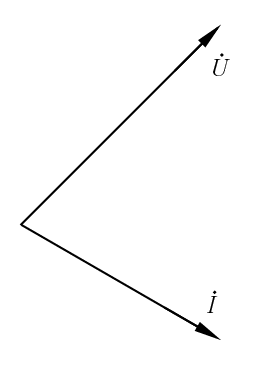
\includegraphics[width=0.172\textwidth]{p11-2-3-sol.png}
\caption*{图 11-2 (3)}
\end{figure}

\paragraph{11-5}\label{11-5}
定性画出题图 11-5 所示各电路的电压、电流相量图。

\begin{figure}[!htb]
\centering
\begin{minipage}[t]{0.231\textwidth}
\centering
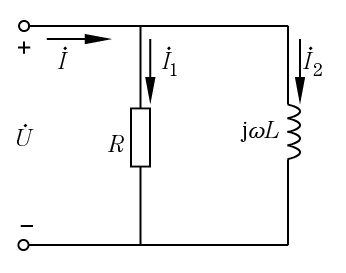
\includegraphics[width=1\textwidth]{p11-5-a.png}
\caption*{(a)}
\end{minipage}
\begin{minipage}[t]{0.236\textwidth}
\centering
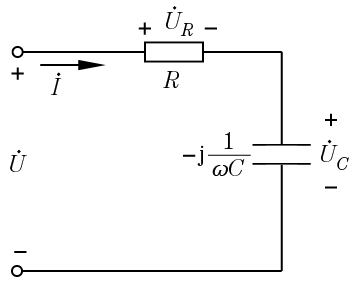
\includegraphics[width=1\textwidth]{p11-5-b.png}
\caption*{(b)}
\end{minipage}
\\
\begin{minipage}[t]{0.218\textwidth}
\centering
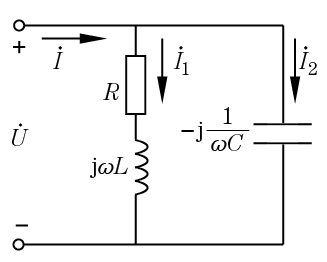
\includegraphics[width=1\textwidth]{p11-5-c.png}
\caption*{(c)}
\end{minipage}
\begin{minipage}[t]{0.251\textwidth}
\centering
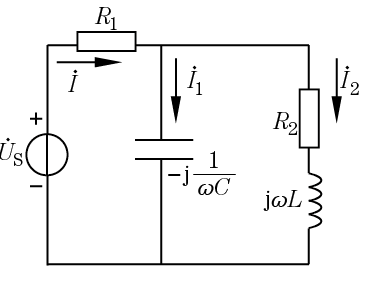
\includegraphics[width=1\textwidth]{p11-5-d.png}
\caption*{(d)}
\end{minipage}
\caption*{题图 11-5}
\end{figure}

\paragraph{解}如图 11-5 所示。

\begin{figure}[!htb]
\centering
\begin{minipage}[t]{0.201\textwidth}
\centering
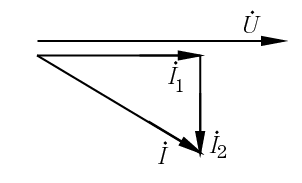
\includegraphics[width=1\textwidth]{p11-5-a-sol.png}
\caption*{(a)}
\end{minipage}
\begin{minipage}[t]{0.191\textwidth}
\centering
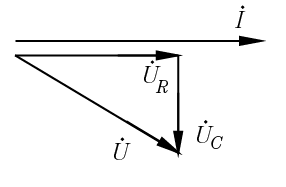
\includegraphics[width=1\textwidth]{p11-5-b-sol.png}
\caption*{(b)}
\end{minipage}
\begin{minipage}[t]{0.144\textwidth}
\centering
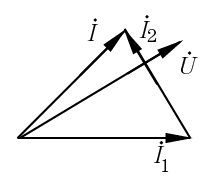
\includegraphics[width=1\textwidth]{p11-5-c-sol.png}
\caption*{(c)}
\end{minipage}
\begin{minipage}[t]{0.143\textwidth}
\centering
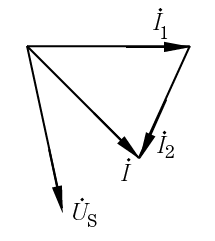
\includegraphics[width=1\textwidth]{p11-5-d-sol.png}
\caption*{(d)}
\end{minipage}
\caption*{图 11-5}
\end{figure}

\paragraph{11-8}\label{11-8}
求题图 11-8 所示各电路的入端阻抗 $Z_{\rm ab}$。

\begin{figure}[!htb]
\centering
\begin{minipage}[t]{0.347\textwidth}
\centering
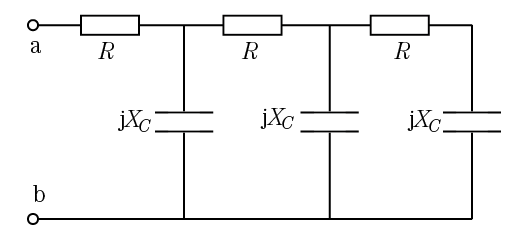
\includegraphics[width=1\textwidth]{p11-8-a.png}
\caption*{(a)}
\end{minipage}
\begin{minipage}[t]{0.243\textwidth}
\centering
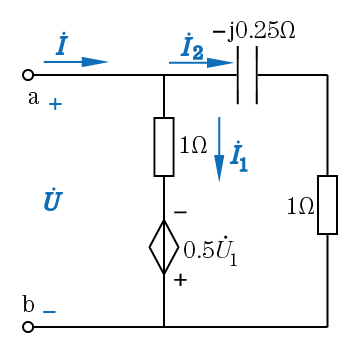
\includegraphics[width=1\textwidth]{p11-8-b.png}
\caption*{(b)}
\end{minipage}
\begin{minipage}[t]{0.312\textwidth}
\centering
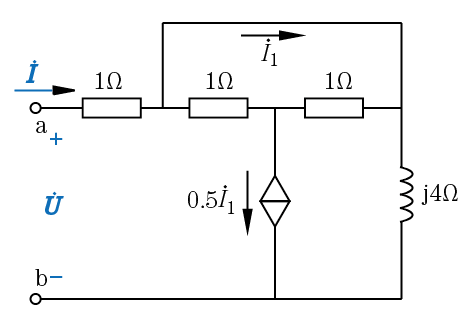
\includegraphics[width=1\textwidth]{p11-8-c.png}
\caption*{(c)}
\end{minipage}
\caption*{题图 11-8}
\end{figure}

\paragraph{解}
(a)
\begin{align*}
Z & = ((\J X_C+R) // \J X_C + R) // \J X_C + R \\
& = \frac{3\J R X_C - X_C^2 + R^2}{R + 2 \J X_C} // \J X_C + R \\
& = \frac{-3 R X_C^2 - \J X_C^3 + \J R^2 X_C}{3 \J R X_C - X_C^2 + R^2 + \J X_C R - 2 X_C^2} + R \\
& = \frac{R^3 - 6 R X_C^2 + \J (5 R^2 X_C - X_C^3)}{R^2 - 3 X_C^2+ \J 4R X_C}
\end{align*}

(b)
$$ \dot {U}_1 = \dot {I}_2 $$
$$ \dot {U} = (1 - \J 0.25) \dot I_2 $$
$$ \dot I_1 = (1.5 - \J 0.25) \dot I_2 $$
$$ \dot I = (2.5 - \J 0.25) \dot I_2 $$
$$ \dot I = \dot I_2 + \dot I_1 = (2.5-\J 0.25) I_2 $$
$$ \therefore R_{\rm eq} = \frac{\dot U}{\dot I} = \frac {1-\J 0.25}{2.5 - \J 0.25} = (0.406 - \J 0.059)\ohm$$

(c)
$$ \dot U = \dot I + (\dot I - \dot I_1) + (\dot I - \dot I_1 - 0.5 \dot I_1) + \J 4 (\dot I - 0.5 \dot I_1) $$
$$  \dot I - \dot I _1 = -( \dot I - \dot I _ 1 - 0.5 \dot I _1)  $$
$$ \therefore  \dot I _1 = 0.8 \dot I  $$
$$ \therefore  \dot U = (1+\J 2.4) \dot I $$
$$  R_{\rm eq} = (1+ \J 2.4)\ohm $$

\paragraph{11-14}\label{11-14}
一线圈接到$U_0=120\volt$的直流电源时,电流$I_0=20\ampere$。若接到频率$f=50\hertz$,电压$U_2=220\volt$的交流电源时,电流$I_2=28.2\ampere$。求此线圈的电阻和电感。

\paragraph{解}
$$ Z = R + \J \omega L $$
$$ R = \frac {U_0}{I_0} = 6 \ohm $$
$$ |I_2| = \frac{|U_2|}{|Z_2|} = \frac{220}{\sqrt{6^2 + (\omega L)^2}} = 28.2, \omega = 2\pi f $$
$$\therefore L = 0.0159 \henry $$

\paragraph{11-20 改}\label{11-20}
电路如题图 11-20 所示。已知$\dot{U}_{\source 1}=100\angle 0\degree \volt$, $\dot{U}_{\source 2}=100\angle -60\degree \volt$, $R_1=R_2=50\ohm$, $X_C=-100\ohm$, $X_L=80\ohm$,求$\dot{I}_1$。

\begin{figure}[!htb]
\centering
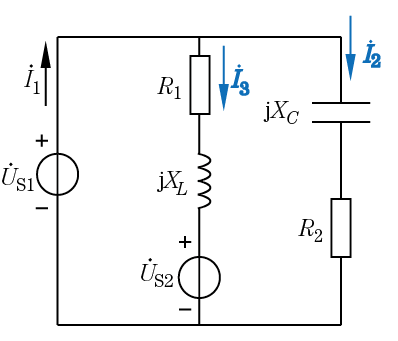
\includegraphics[width=0.265\textwidth]{p11-20.png}
\caption*{题图 11-20}
\end{figure}

\paragraph{解}
 $$ \dot I _2 = \frac{ \dot U _{\source 1}}{ \J X_C + R_2} = (0.4 + \J 0.8) \ampere $$
 $$ \dot I _3 = \frac{ \dot U _{\source 1}- \dot U _{\source 2}}{R_1 + \J X_L} = (1.06 + \J 0.037) \ampere $$
 $$ \therefore \dot I = (1.46+ \J 0.837)\ampere = 1.682\angle 29.8 \degree \ampere $$

\paragraph{11-23}\label{11-23}
题图 11-23 所示电路为一种移相电路。用相量分析说明改变电阻可使电压$\dot{U}_{\rm ab}$相位变化而大小不变。若$U=2\volt$, $f=200\hertz$, $R_1=4\kiloohm$, $C=0.01\microfarad$, $R_2$由$30\kiloohm$变至$140\ohm$,求$\dot{U}_{\rm ab}$的相位变化。

\begin{figure}[!htb]
\centering
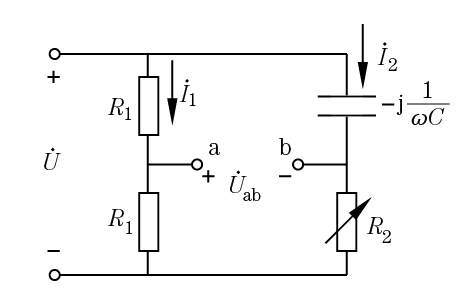
\includegraphics[width=0.315\textwidth]{p11-23.png}
\caption*{题图 11-23}
\end{figure}

\paragraph{解}设$\dot {U}$的负极处为电势零点。
 $$ \dot U _{\rm a} = \frac{1}{2} \dot U $$
 $$ \dot U _{\rm b} = \frac{ \dot U }{R_2 - \J \frac{1}{\omega C}} \cdot R_2 = \frac { \dot U R_2 \omega C} {R_2 \omega C - \J } $$
 $$ \dot U _{\rm ab} = \frac { \dot U }{2} - \frac { \dot U R_2 \omega C} {R_2 \omega C - \J } = \frac{ \dot U }{2} \cdot \frac{ \J + R_2 \omega C}{ \J - R_2 \omega C} $$
 $$ \therefore | \dot U _{\rm ab} | = | \frac{ \dot U }{2} |,\dot U _{\rm ab} \text{相位变化而大小不变}$$
 $ U = 2 \volt, f = 200 \hertz, R_1 = 4 \kiloohm, C = 0.01 \microfarad $, 记 $ \dot U = 2 \angle 0 \degree \volt $\\
 $R_2 = 30 \kiloohm$时,$\dot U_{\rm ab} = 1 \angle -41.31 \degree$。\\
 $R_2 = 140 \ohm$时,$\dot U_{\rm ab} = 1 \angle -0.201 \degree$。\\
 $\therefore \Delta \varphi = 41.1 \degree$ \\
 (疑为题目有误,$R_2 = 140 \kiloohm$时,$\dot U_{\rm ab} = 1 \angle -120.78 \degree$,$\Delta \varphi = -79.4 \degree$)

\paragraph{11-28}\label{11-28}
分别用回路法和节点法列写题图 11-28 所示电路的相量方程。

\begin{figure}[!htb]
\centering
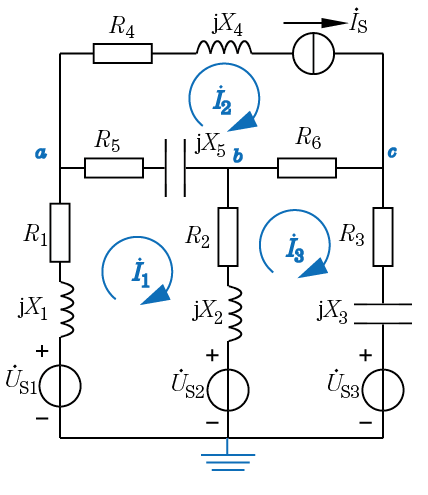
\includegraphics[width=0.285\textwidth]{p11-28.png}
\caption*{题图 11-28}
\end{figure}

\paragraph{解}

\subparagraph{回路电流法}
\begin{align*}
\left\{ \begin{aligned}
 - \dot U _{\source 1}+ \dot I _1(R_1+ \J X_1)+( \dot I _1- \dot I _2)(R_5+ \J X_5) + ( \dot I _1- \dot I _3)(R_2+ \J X_2) + \dot U _{\source 2} & = 0 \\
 - \dot U _{\source 2}+( \dot I _3- \dot I _1)( \J X_2+R_2)-( \dot I _3- \dot I _2)R_6+ \dot I _3(R_3+ \J X_3)+ \dot U _{\source 3} & = 0 \\
 \dot I _2 & = \dot I _\source
\end{aligned} \right.
\end{align*}

\subparagraph{节点电压法}
\begin{align*} \left\{ \begin{aligned}
 \frac{ \dot U _a - \dot U _{\source 1}}{R_1 + \J X_1} + \frac{ \dot U _a - \dot U _b}{R_5 + \J X_5} + \dot I _\source & = 0 \\
 \frac{ \dot U _b- \dot U _a}{R_5+ \J X_5} + \frac{ \dot U _b - \dot U _{\source 2}}{R_2 + \J X_2} + \frac{ \dot U _b - \dot U _c}{R_6} & = 0 \\
 \frac{ \dot U _c - \dot U _b}{R_6} + \frac{ \dot U _c - \dot U _{\source 3}} {R_3 + \J X_3} - \dot I _\source & = 0
\end{aligned} \right. \end{align*}

\paragraph{11-30}\label{11-30}
电路如题图 11-30 所示。已知$U=220\volt$, $Z_2=15+\J 20\ohm$, $Z_3=20\ohm$, $\dot{I}_2=4\angle 0\degree \ampere$, 且$\dot{I}_2$滞后$\dot{U}$ $30\degree$,求$Z_1$。

\begin{figure}[!htb]
\centering
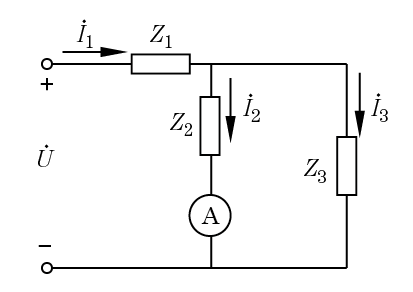
\includegraphics[width=0.275\textwidth]{p11-30.png}
\caption*{题图 11-30}
\end{figure}

\paragraph{解}由$\dot I_2 = 4 \angle 0 \degree \ampere$且滞后$\dot U$ $30 \degree$知
 $$ \dot U = 220 \angle 30 \degree \volt $$
 $$ \dot U _{Z1} = \dot U - \dot I _2 Z_2 = 133.93 \angle 12.94 \degree \volt $$
 $$ \dot I _3 = \frac{ \dot I _2 Z_2}{Z_3} = 5 \angle 53.13 \degree \ampere $$
 $$ \dot I _1 = \dot I _3 + \dot I _2 = 8.06 \angle \degree 29.74 \degree \ampere $$
 $$ Z_1 = \frac{ \dot U _{Z1}}{ \dot I _1} = 16.61 \angle -16.80 \degree \ohm = (15.90 - \J 4.80) \ohm $$

\paragraph{11-32}\label{11-32}
在同一相量图中,定性画出题图 11-32 所示电路中各元件电压、电流的相量关系。

\begin{figure}[!htb]
\centering
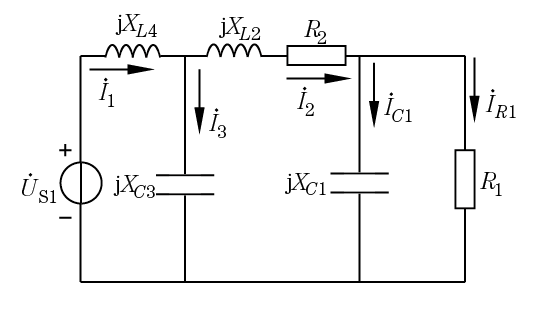
\includegraphics[width=0.367\textwidth]{p11-32.png}
\caption*{题图 11-32}
\end{figure}

\paragraph{解}
如图所示,其中$\dot I_{R1}$与$\dot U_{C1}$垂直,$\dot I_{2}$与$\dot U_{L2}$垂直,$\dot I_{3}$与$\dot U_{C3}$垂直,$\dot I_{4}$与$\dot U_{L4}$垂直。

\begin{figure}[!htb]
\centering
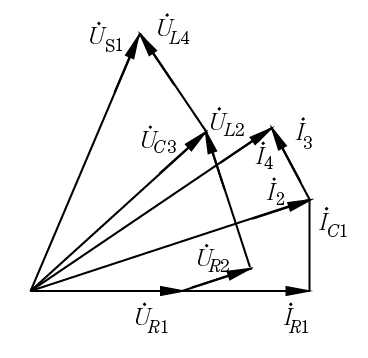
\includegraphics[width=0.245\textwidth]{p11-32-sol.png}
\caption*{图 11-32}
\end{figure}

\paragraph{11-39}\label{11-39}
电路如图11-39所示,$R_1=6\ohm$, $R_2=2\ohm$, $R_3=1\ohm$, $\dot{I}_\source=10\angle 0\degree \ampere$, $\dot{U}_\source=30\angle 0\degree \volt$, $\J X_C=-\J 3\ohm$, $\J X_L = \J 6\ohm$。用戴维南定理求图中电流$\dot{I}$。

\begin{figure}[!htb]
\centering
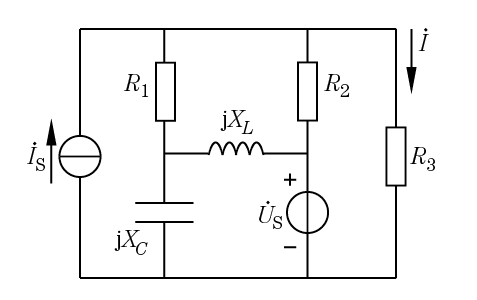
\includegraphics[width=0.318\textwidth]{p11-39.png}
\caption*{题图 11-39}
\end{figure}

\paragraph{解} 如图 11-39 所示,求$R_3$以外部分的戴维南等效电路。则

\begin{figure}[!htb]
\centering
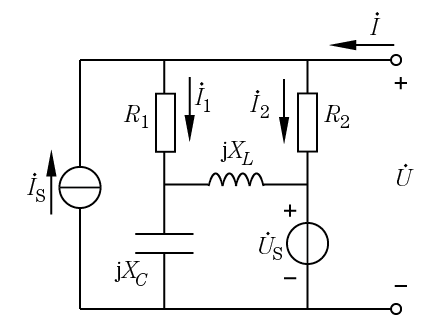
\includegraphics[width=0.294\textwidth]{p11-39-sol.png}
\caption*{图 11-39}

\end{figure}
 $$ \dot I _2 = \frac{ \dot U -30}{2} $$
 $$ \therefore \dot I _1 = \dot I - \frac{ \dot U -30}{2} + 10 = \dot I - \frac{ \dot U }{2} + 25 $$
 $$ \therefore \dot U _C = \dot U - 6 \dot I _1 = 4 \dot U - 6 \dot I - 150 $$
 $$ \because \frac{ \dot U _C - 30}{ \J 6} + \frac{ \dot U _C}{- \J 3} = \dot I _1 $$
 $ \therefore \text{代入} \dot U _C, \dot I _1$ 得
 $$ (-4+ \J 3) \dot U = (-6+ \J 6) \dot I +(-120+ \J 150) $$
 $$ \therefore \dot U_{\rm eq}=(37.2-\J 9.6) \volt, R_{\rm eq} = (1.68 - \J 0.24) \ohm $$
 $$ \therefore \dot U = (1.68 - \J 0.24) \dot I +(37.2-\J 9.6) $$
 $$  \dot I = \frac{ \dot U _{\rm eq}}{R_{\rm eq}+1} = (14.09 - \J 2.32) \ampere = 14.28\angle -9.4 \degree \ampere $$

\paragraph{11-51}\label{11-51}
题图 11-51(a) 所示电路中,$\dot{U}_1=220 \angle 0 \degree \volt$, $\dot{I}_1 = 5 \angle -30 \degree \ampere$, $\dot{U}_2 = 110 \angle -45 \degree \volt$。图(b)中,$\dot{I}_2'=10\angle 0\degree \ampere$, 阻抗$Z_1=(40+\J 30)\ohm$, 则$Z_1$中电流$\dot{I}_1'$为多大?

\begin{figure}[!htb]
\centering
\begin{minipage}[t]{0.291\textwidth}
\centering
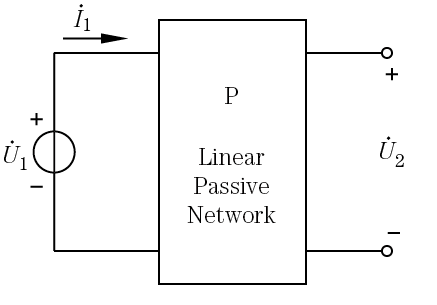
\includegraphics[width=1\textwidth]{p11-51-a.png}
\caption*{(a)}
\end{minipage}
\begin{minipage}[t]{0.327\textwidth}
\centering
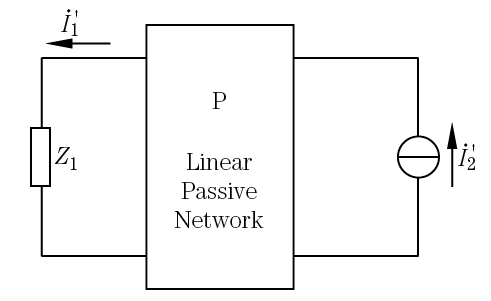
\includegraphics[width=1\textwidth]{p11-51-b.png}
\caption*{(b)}
\end{minipage}
\caption*{题图 11-51}
\end{figure}

\paragraph{解}设(a)中$\rm P$的各个支路电压、电流为$\dot U_i, \dot I_i (i=3,4,5,\cdots,n)$(取关联参考方向,下同),(b)中对应者为$\dot U_i', \dot I_i' $。\\
由特勒根定理
\begin{align*}
\left\{ \begin{aligned}
 \dot U _1 \dot I _1'+ \dot U _2(- \dot I _2') + \sum_{i=3}^{n} \dot U _i \dot I _i' &= 0 \\
 (Z_1 \dot I _1')(- \dot I _1') + \dot U _2' \cdot 0 + \sum_{i=3}^{n} \dot U _i' \dot I _i &= 0 \\
\end{aligned} \right.
\end{align*}
由于$\rm P$为无源线性网络,则
 $$ \dot U _i \dot I _i' = R_i \dot I _i \dot I _i' = \dot U _i' \dot I _i$$
从而两式相减化简可得
 $$ \dot U _1 \dot I _1' - \dot U _2 \dot I _2' = Z_1 \dot I _1'(- \dot I _1) $$
 $$ \therefore \dot I _1' = \frac{ \dot U _2 \dot I _2'}{ \dot U _1+Z_1 \dot I _1} = (1.549 - \J 1.760) \ampere = 2.34 \angle -48.7 \degree \ampere $$

\paragraph{11-53 改}\label{11-53}
题图 11-53 所示电路中,已知$I_\source = 1\ampere$,当$X_L=2\ohm$时,测得电压$U_{\rm AB}=2\volt$;当$X_L=4\ohm$时,测得电压仍为$U_{\rm AB}=2\volt$。试确定电阻$R$以及容抗$X_C$的值。

\begin{figure}[!htb]
\centering
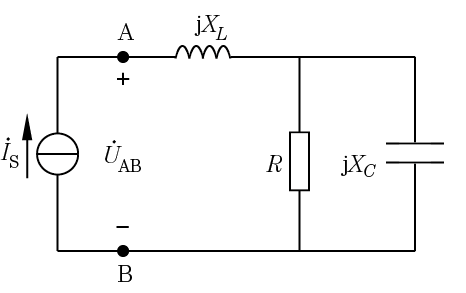
\includegraphics[width=0.311\textwidth]{p11-53.png}
\caption*{题图 11-53}
\end{figure}

\paragraph{解}
$$ \dot U _{\rm AB} = \dot I _\source \left( \J X_L + \frac{ \J RX_C}{R+ \J X_C} \right) = \J X_L + \frac{ \J RX_C}{R+ \J X_C} $$
设 $\frac{ \J RX_C}{R+ \J X_C} = a + \J b$, 由于是电容和电阻并联,则$b<0, a>0$,且由题中数据可知
\begin{align*}
\left\{ \begin{aligned}
\left| a+(2+b) \J \right| & = 2 \\
\left| a+(4+b) \J \right| & = 2
\end{aligned} \right. 
\end{align*}
$$ \therefore b = -3, a = \sqrt{3} $$
$$ \therefore X_C = -4 \ohm, R = 4\sqrt{3} \ohm $$
\end{document} 